\beginsong{Notabene}[wuw={Carl Michael Bellmann, im deutschen von Klabund, zwischen 1740 und 1795}, bo={186}, index={Holt mir Wein aus vollen Krügen}]

\markboth{\songtitle}{\songtitle}

\beginverse
\endverse

\centering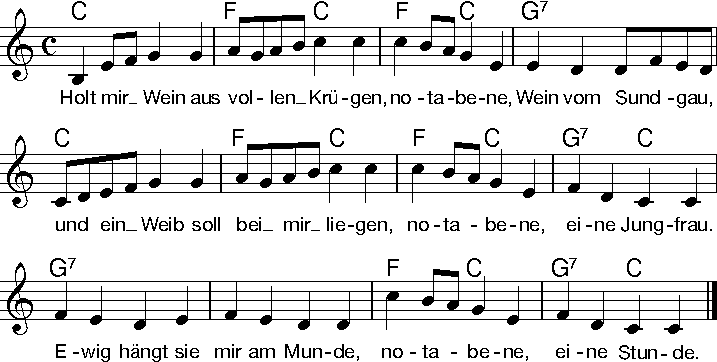
\includegraphics[width=1\textwidth]{Noten/Lied073.pdf}	

\beginverse
\[C]Ach, das Leben \[F]lebt sich \[C]lyrisch, \[F]nota\[C]bene, \[G7]wenn man jung ist
\[C]und es duftet \[F]gar ver\[C]führisch, \[F]nota\[C]bene, \[G7]wenn's kein \[C]Dung ist.
\[G7]Ach wie leicht wird hier erreicht doch, \[F]nota\[C]bene, \[G7]ein 'Viel\[C]leicht' noch.
\endverse

\beginverse
^Lasst die Erde ^heiß sich ^drehen, ^nota^bene, ^bis sie kalt ist.
^Deine Liebste ^sollst du ^sehen, ^nota^bene, ^wenn sie ^alt ist.
^Lache, saufe, hure, trabe, ^nota^bene, ^bis zum ^Grabe.
\endverse
 
\endsong

\beginscripture{} 
Nota bene ist eine lateinische und italienische Floskel, die mit „wohlgemerkt“, „merke wohl „beachte wohl“ oder auch „übrigens“ übersetzt werden kann. Sie leitet sich vom lateinischen Verb notare ab, aus dem auch das deutsche Wort 'notieren' entstanden ist.
\newpage
\endscripture

\begin{intersong}


\ifthenelse{\boolean{pics}}{
\vspace{100pt}
\centering
\includegraphics[width=0.75\textwidth]{Bilder/wein.png}	
}{}

\end{intersong}